\documentclass[11pt,a4paper]{article}

\usepackage[english]{babel}
\usepackage[T1]{fontenc}
\usepackage[utf8]{inputenc}

% Math essentials
\usepackage{amsmath, amssymb}
\usepackage{bm}

% Units and hyperlinks
\usepackage{siunitx}
\sisetup{per-mode=symbol}

\usepackage{natbib}
\usepackage{graphicx}
\usepackage{lmodern}
\usepackage{caption}
\usepackage{subcaption}
\usepackage{float}
\usepackage{url}
\usepackage{titlepic}
\usepackage{listings}
\usepackage{nameref}
\usepackage{xcolor}
\usepackage{array}
\setlength{\marginparwidth}{2cm}
\usepackage{todonotes}
\usepackage{datetime}
\usepackage{parskip}
\usepackage{hyperref}

% ------- Macros defined in this document -------
\newcommand{\vect}[1]{\bm{#1}}       % bold italic vectors
\newcommand{\mat}[1]{\mathbf{#1}}    % bold upright matrices
\newcommand{\trans}{\mathsf{T}}      % transpose, use as ^{\trans}

% \newcommand{\SO}{\mathrm{SO}}
% \newcommand{\SE}{\mathrm{SE}}

\newcommand{\skewsym}[1]{\left[#1\right]_\times}

\newcommand{\SkewFrom}[3]{%
  \begin{bmatrix}
    0 & -#3 & #2 \\
    #3 & 0 & -#1 \\
    -#2 & #1 & 0
  \end{bmatrix}%
}

\title{Ground Vehicle Robot Kinematics}
% \author{ \includegraphics[width=0.5\linewidth]{images/logo.jpg} }
\author{Juan Francisco Rasc\'on Crespo}
\date{\today}

\setcounter{secnumdepth}{2}
\setcounter{tocdepth}{2}

\begin{document}
\maketitle

% \thispagestyle{empty}
% \newpage

% \tableofcontents
% \newpage

\section{Wheel Constraints}
\todo[inline]{Complete}

\section{Base with Three Active Steerable Wheels (Three Swerve Drive)}
% \subsection{AGV Simulation}
% \label{sec:state-machine}

A base with three active steerable wheels (three swerve drive) is an omnidirectional locomotion system. It allows a ground robot to move in any direction without first changing the chassis orientation. Each wheel is oriented independently, which gives the robot maneuverability and flexibility.

\begin{figure}[H]
\centering
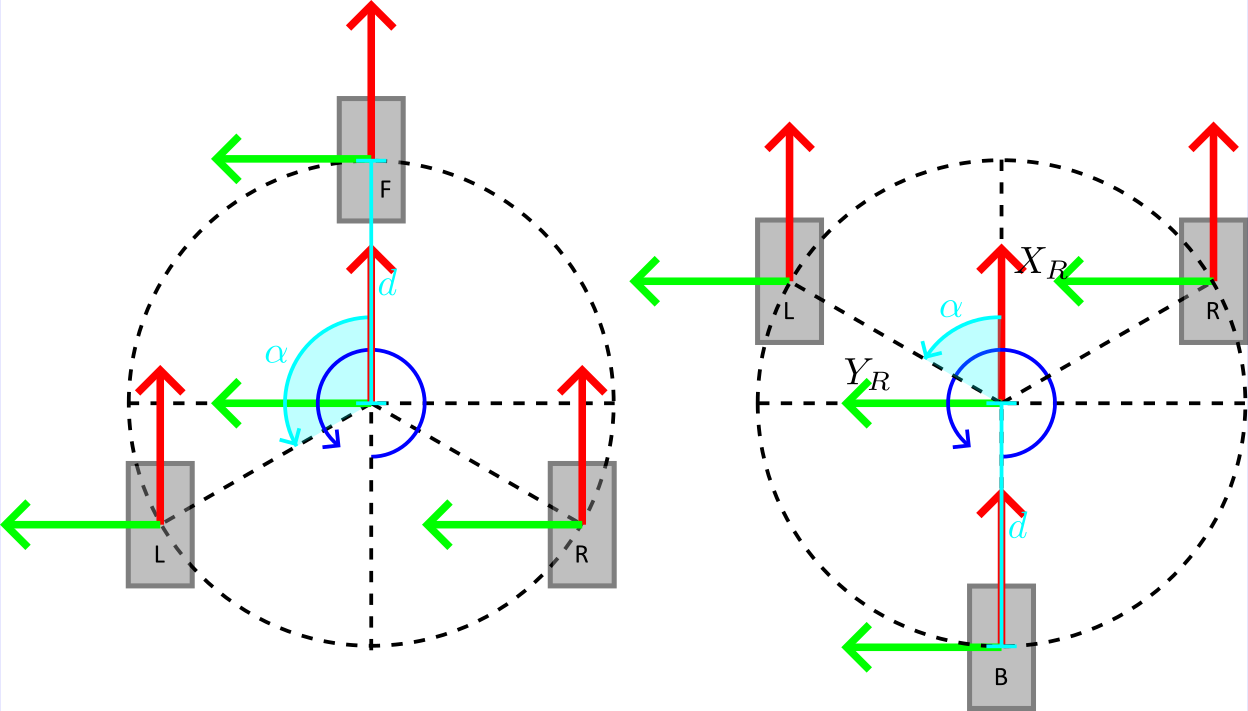
\includegraphics[width=1.0\linewidth]{images/three_drive_configuration.png}
\caption{Common wheel configurations in a three swerve drive system (left: inverted-Y configuration, right: Y configuration)}
\label{fig:three-swerve-drive-configuration}
\end{figure}

The typical wheel layout is triangular. The two most common configurations are:

\begin{itemize}
\item Inverted-Y configuration: One wheel is placed at distance $d$ from the center on the positive $X_R$ axis. The other two are also placed at distance $d$, at angles $\alpha^\circ$ and $-\alpha^\circ$ with respect to the positive $X_R$ axis, with $\alpha \in [90^\circ, 180^\circ)$.
\item Y configuration: One wheel is placed at distance $d$ from the center on the negative $X_R$ axis. The other two are also placed at distance $d$, at angles $\alpha^\circ$ and $-\alpha^\circ$ with respect to the positive $X_R$ axis, with $\alpha \in (0^\circ, 90^\circ]$.
\end{itemize}

Figure \ref{fig:three-swerve-drive-configuration} shows both configurations.

The following sections present inverse and forward kinematics for a robot with three active wheels under the previous configurations. A more general formulation can also be considered, with different distances to the center or wheel angles that are not symmetric. However, those configurations are less common and, in this context, only complicate the expressions without practical advantages, since in industry the previously described configurations are predominantly used.

For the inverted-Y configuration, $i \in \{F,L,R\}$ is used to identify each wheel.
For the Y configuration, $i \in \{B,L,R\}$ is used.

The base linear velocity is denoted as:
\begin{equation}
\vect{V} = \begin{bmatrix} V_x \\ V_y \\ 0 \end{bmatrix}
\label{eq:rigid-velocity}
\end{equation}
and is expressed in \si{\meter\per\second}.

The base angular velocity is denoted as:
\begin{equation}
\boldsymbol{\omega} = \begin{bmatrix} 0 \\ 0 \\ \omega_z \end{bmatrix}
\label{eq:rigid-angular-velocity}
\end{equation}

The linear velocity of each wheel $i$ is expressed as:
\begin{equation}
\begin{aligned}
\vect{V}_i &= \vect{V} + \vect{\omega} \times \vect{d}_i \\
           &= \vect{V} + \skewsym{\boldsymbol{\omega}}\,\vect{d}_i
\end{aligned}
\label{eq:wheel-velocity}
\end{equation}
where $\vect{d}_i$ is the position vector of wheel $i$ with respect to the base center.

The cross product between $\boldsymbol{\omega}$ and $\vect{d}_i$ can be written as a matrix product through the skew-symmetric operator $[\cdot]_{\times}$:
$\boldsymbol{\omega} \times \vect{d}_i = \skewsym{\boldsymbol{\omega}}\,\vect{d}_i$, and
$\skewsym{\boldsymbol{\omega}}$ is defined as:
\[
\skewsym{\boldsymbol{\omega}} \triangleq
\SkewFrom{\omega_x}{\omega_y}{\omega_z}
\]

Therefore, considering $\boldsymbol{\omega}=\begin{bmatrix}0&0&\omega_z\end{bmatrix}^{\trans}$ and $\vect{d}_i=\begin{bmatrix}d\cos\alpha_i&d\sin\alpha_i&0\end{bmatrix}^{\trans}$:
\begin{equation}
\vect{V}_i
= \vect{V}
+ \begin{bmatrix}
-\omega_z d\sin\alpha_i \\
\omega_z d\cos\alpha_i \\
0
\end{bmatrix}
= \begin{bmatrix}
V_x - \omega_z d\sin\alpha_i \\
V_y + \omega_z d\cos\alpha_i \\
0
\end{bmatrix}
\label{eq:wheel-velocity-expanded}
\end{equation}

The magnitude of the linear velocity of each wheel $i$ is given by:
\begin{equation}
\begin{aligned}
\|\vect{V}_i\| = \sqrt{(V_x - \omega_z d\sin\alpha_i)^2 + (V_y + \omega_z d\cos\alpha_i)^2} = \omega_i r
\end{aligned}
\label{eq:wheel-speed}
\end{equation}

where $r$ is the wheel radius and $\omega_i$ is the angular speed of wheel $i$.

Obviously, all wheels have the same radius $r$.

\subsection{Inverse Kinematics}

Inverse kinematics is the process of computing wheel angular speeds $\omega_i$ and steering angles $\theta_i$ from the base linear velocity $\vect{V}$ and base angular velocity $\boldsymbol{\omega}$.

The orientation of each wheel $i$, $\theta_i$, is obtained from its linear velocity $\vect{V}_i$:
\begin{equation}
\theta_i = \arctan2(V_{iy}, V_{ix}) = \arctan2(V_y + \omega_z d\cos\alpha_i, V_x - \omega_z d\sin\alpha_i)
\label{eq:inverse-kinematics-angle}
\end{equation}

Then, the angular speed of each wheel $i$, $\omega_i$, is obtained from its linear velocity $\vect{V}_i$ and radius $r$:
\begin{equation}
\omega_i = \frac{\|\vect{V}_i\|}{r} = \frac{\sqrt{(V_x - \omega_z d\sin\alpha_i)^2 + (V_y + \omega_z d\cos\alpha_i)^2}}{r}
\label{eq:inverse-kinematics-speed}
\end{equation}


\begin{figure}[H]
\centering
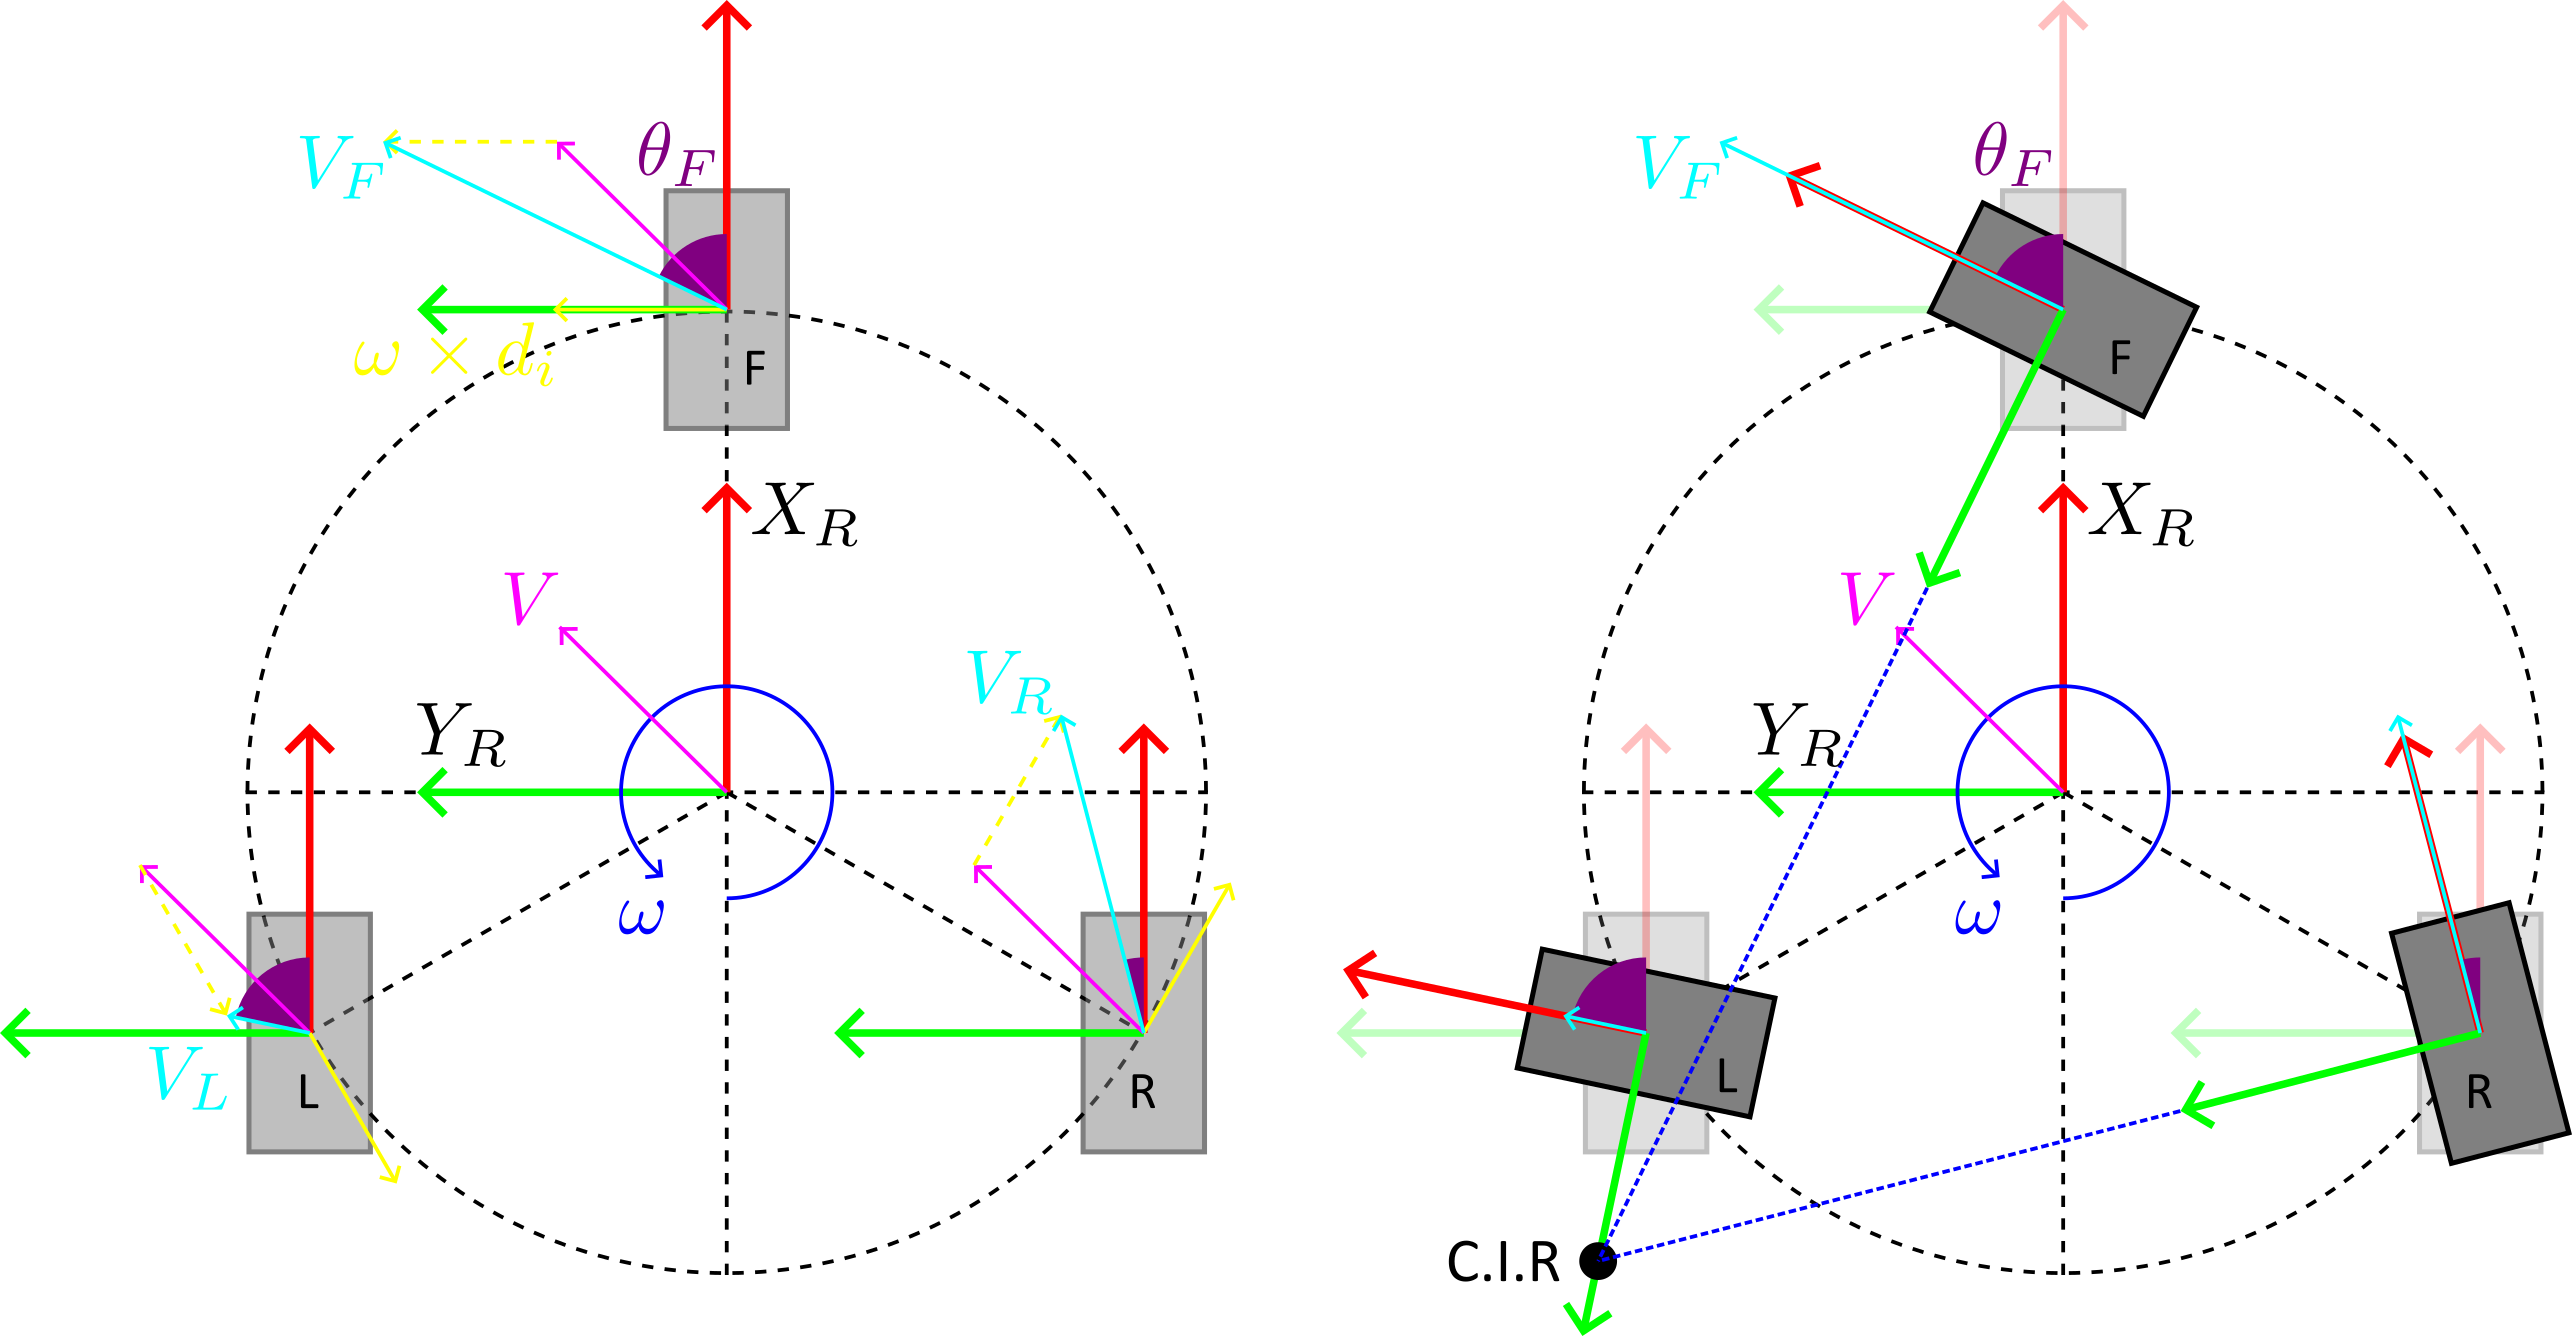
\includegraphics[width=1.0\linewidth]{images/inverted_y_inverse_kinematics.png}
\caption{Inverse kinematics of a robot with inverted-Y configuration}
\label{fig:inverted-y-inverse-kinematics}
\end{figure}

\begin{figure}[H]
\centering
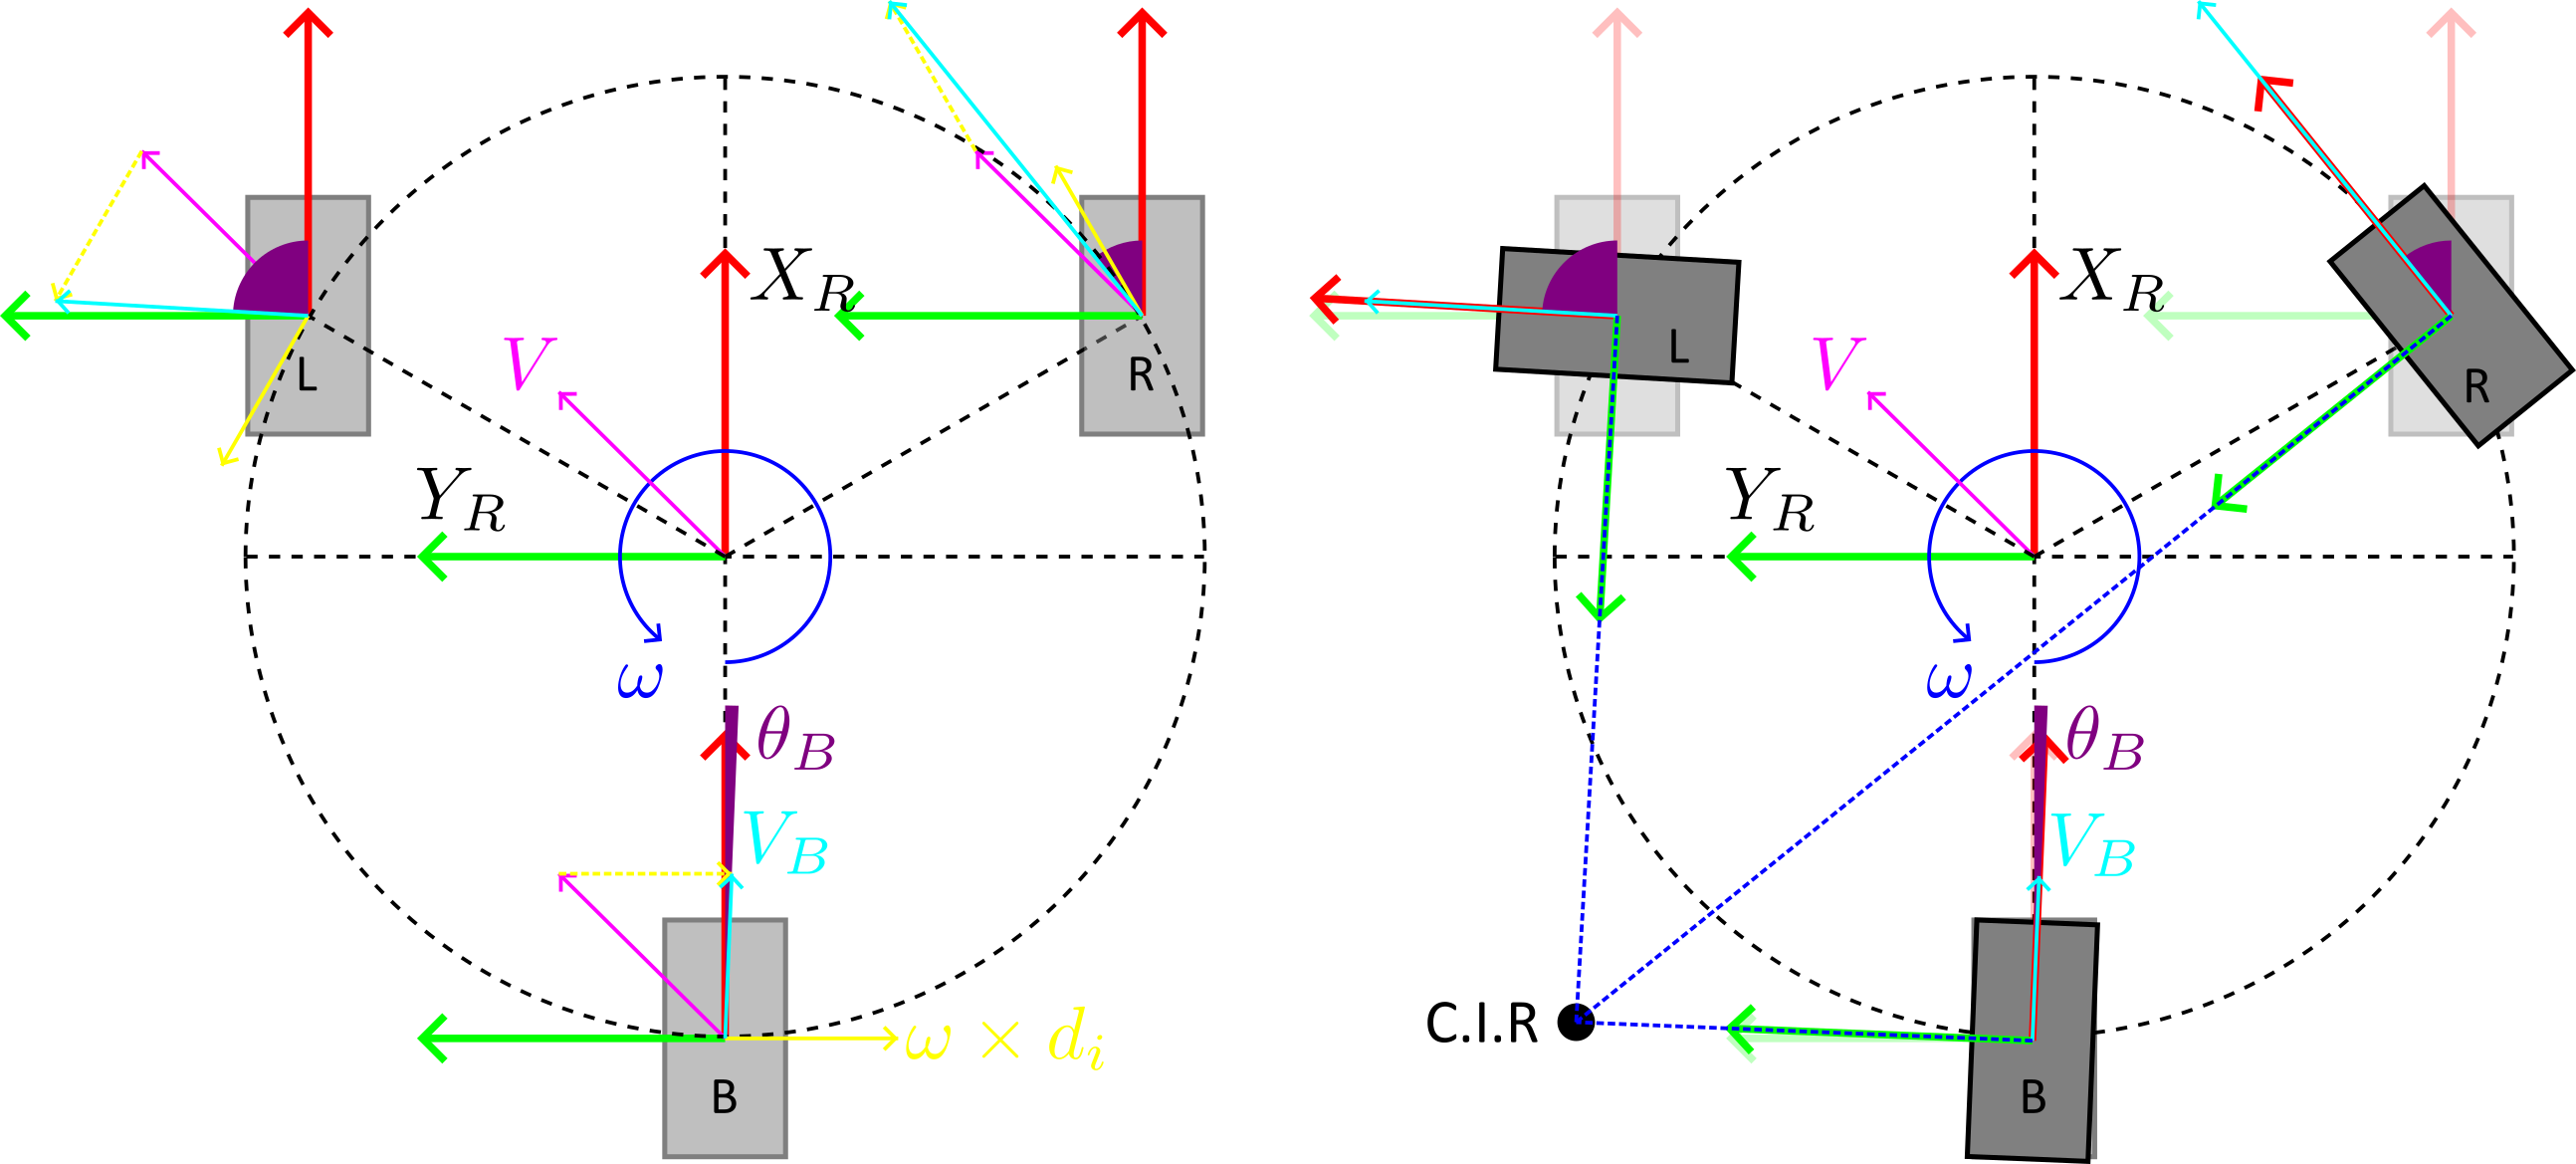
\includegraphics[width=1.0\linewidth]{images/y_inverse_kinematics.png}
\caption{Inverse kinematics of a robot with Y configuration}
\label{fig:y-inverse-kinematics}
\end{figure}

\subsection{Forward Kinematics}

Forward kinematics is the process of computing the base linear velocity $\vect{V}$ and base angular velocity $\boldsymbol{\omega}$ from wheel angular speeds $\omega_i$ and wheel orientations $\theta_i$.

There are 6 input variables: wheel angular speeds $\omega_i$ and orientations $\theta_i$ for each wheel $i$. The goal is to compute 3 output variables: base linear velocity $\vect{V} = (V_x, V_y, 0)^{\mathsf{T}}$ and base angular velocity $\boldsymbol{\omega} = (0, 0, \omega_z)^{\mathsf{T}}$. Therefore, the system is overdetermined and is robustly solved using least squares.
For the inverted-Y configuration, $i \in \{F,L,R\}$ is used (Front, Left, Right). For the Y configuration, this becomes $i \in \{B,L,R\}$ (Back, Left, Right).

For each wheel $i$, define the rolling unit vector:
\begin{equation}
\vect{t}_i = \begin{bmatrix}
\cos\theta_i \\
\sin\theta_i \\
0
\end{bmatrix}
\label{eq:wheel-rolling-direction}
\end{equation}

The linear velocity of the wheel along its rolling direction is:
\begin{equation}
\vect{V}_i = r\omega_i \vect{t}_i
= r\omega_i
\begin{bmatrix}
\cos\theta_i \\
\sin\theta_i \\
0
\end{bmatrix}
\label{eq:wheel-linear-from-omega}
\end{equation}

By equating \eqref{eq:wheel-velocity-expanded} and \eqref{eq:wheel-linear-from-omega}, for each wheel $i$:
\begin{equation}
\begin{aligned}
V_x - \omega_z d\sin\alpha_i &= r\omega_i\cos\theta_i \\
V_y + \omega_z d\cos\alpha_i &= r\omega_i\sin\theta_i
\end{aligned}
\label{eq:direct-kinematics-per-wheel}
\end{equation}

In the ideal case (no noise and no slip), any subset of 3 independent equations allows solving $\vect{V}$ and $\vect{\omega}$ exactly.
From an ideal mathematical point of view, the procedure is to build a linear system and solve it with least squares.

\begin{equation}
A\mathbf{x}=\mathbf{b},
\quad
\mathbf{x}=
\begin{bmatrix}
V_x\\
V_y\\
\omega_z
\end{bmatrix}
\label{eq:direct-linear-system}
\end{equation}

\begin{equation}
\hat{\mathbf{x}}
= \arg\min_{\mathbf{x}}\|A\mathbf{x}-\mathbf{b}\|_2^2
= (A^{\mathsf{T}}A)^{-1}A^{\mathsf{T}}\mathbf{b}
\label{eq:direct-least-squares}
\end{equation}

As reference, for the inverted-Y configuration (\(i\in\{F,L,R\}\)) the following matrices $A$ and $\mathbf{b}$ are used:
\begin{equation}
A_{\text{inverted-Y}}=
\begin{bmatrix}
1 & 0 & -d\sin\alpha_F\\
0 & 1 & \phantom{-}d\cos\alpha_F\\
1 & 0 & -d\sin\alpha_L\\
0 & 1 & \phantom{-}d\cos\alpha_L\\
1 & 0 & -d\sin\alpha_R\\
0 & 1 & \phantom{-}d\cos\alpha_R
\end{bmatrix}
\label{eq:A-y-invertida}
\end{equation}
\begin{equation}
\mathbf{b}_{\text{inverted-Y}}
=r\begin{bmatrix}
\omega_F\cos\theta_F\\
\omega_F\sin\theta_F\\
\omega_L\cos\theta_L\\
\omega_L\sin\theta_L\\
\omega_R\cos\theta_R\\
\omega_R\sin\theta_R
\end{bmatrix}
\label{eq:b-y-invertida}
\end{equation}

with $\alpha_F=0^\circ$, $\alpha_L=\alpha$, and $\alpha_R=-\alpha$.

For the Y configuration (\(i\in\{B,L,R\}\)) the following matrices $A$ and $\mathbf{b}$ are used:
\begin{equation}
A_{\text{Y}}=
\begin{bmatrix}
1 & 0 & -d\sin\alpha_B\\
0 & 1 & \phantom{-}d\cos\alpha_B\\
1 & 0 & -d\sin\alpha_L\\
0 & 1 & \phantom{-}d\cos\alpha_L\\
1 & 0 & -d\sin\alpha_R\\
0 & 1 & \phantom{-}d\cos\alpha_R
\end{bmatrix}
\label{eq:A-y}
\end{equation}
\begin{equation}
\mathbf{b}_{\text{Y}}
=r\begin{bmatrix}
\omega_B\cos\theta_B\\
\omega_B\sin\theta_B\\
\omega_L\cos\theta_L\\
\omega_L\sin\theta_L\\
\omega_R\cos\theta_R\\
\omega_R\sin\theta_R
\end{bmatrix}
\label{eq:b-y}
\end{equation}

with $\alpha_B=180^\circ$, $\alpha_L=\alpha$, and $\alpha_R=-\alpha$.

Note that the least-squares solution in \eqref{eq:direct-least-squares} is valid whenever $A^{\mathsf{T}}A$ is invertible.

In real conditions, the 6 equations do not match exactly due to several causes:
\begin{itemize}
\item sensor noise
\item wheel slip
\item geometry or calibration errors
\item encoder quantization
\end{itemize}

Although the closed-form expression \eqref{eq:direct-least-squares} is useful for analysis, in numerical implementation it is recommended to avoid explicit computation of $(A^{\mathsf{T}}A)^{-1}$, since for the causes above $A$ can be ill-conditioned or even singular, which can make $A^{\mathsf{T}}A$ non-invertible or its inverse numerically unstable.

From an implementation point of view, the recommended approach is to solve least squares with numerically stable methods, instead of using explicit inversion of $(A^{\mathsf{T}}A)$.

Two approaches can be followed:
\begin{itemize}
\item Solve the least-squares problem directly via QR decomposition (orthogonal-triangular decomposition).
\item Solve it via the Moore-Penrose pseudoinverse:
\[
\hat{\mathbf{x}} = A^{\dagger}\mathbf{b}
\]
In this approach, the usual way to compute $A^{\dagger}$ robustly is singular value decomposition (SVD).
\end{itemize}

As a practical implementation criterion:
\begin{itemize}
\item \textbf{QR (orthogonal-triangular decomposition):}
\begin{itemize}
\item Advantages: lower computational cost and higher speed.
\item Drawback: lower robustness when the system is highly ill-conditioned or nearly singular.
\item Recommended use: online estimation of $\hat{\mathbf{x}}$ when the problem is reasonably well-conditioned.
\end{itemize}

\item \textbf{SVD (singular value decomposition):}
\begin{itemize}
\item Advantages: higher numerical robustness and better handling of ill-conditioned or nearly singular systems; it also allows diagnosis of the effective rank of the system.
\item Drawback: higher computational cost.
\item Recommended use: when numerical stability and robustness against noise or poor conditioning are prioritized.
\end{itemize}
\end{itemize}

To choose between QR and SVD in this problem, the following procedure can be used:
\begin{itemize}
\item Build $A$ from geometry ($d$ and $\alpha_i$).
\item Evaluate its conditioning once (for example, at startup), since $A$ is constant if the geometry does not change.
\item Compute the condition number of $A$:
\[
\kappa(A)=\frac{\sigma_{\max}(A)}{\sigma_{\min}(A)}
\]
where $\sigma_{\max}(A)$ and $\sigma_{\min}(A)$ are, respectively, the largest and smallest singular values of $A$.
\begin{itemize}
\item To obtain singular values, use singular value decomposition:
\[
A=U\Sigma V^{\mathsf{T}}
\]
where $U$ and $V$ are orthogonal matrices, and $\Sigma$ is a diagonal (or rectangular-diagonal) matrix whose diagonal elements are the singular values $\sigma_i$.
\item Equivalent practical form:
\begin{itemize}
\item Compute $A^{\mathsf{T}}A$.
\item Obtain its eigenvalues $\lambda_i$.
\item Compute $\sigma_i=\sqrt{\lambda_i}$.
\item Compute explicitly:
\[
\sigma_{\max}=\sqrt{\lambda_{\max}(A^{\mathsf{T}}A)},
\quad
\sigma_{\min}=\sqrt{\lambda_{\min}(A^{\mathsf{T}}A)}
\]
\end{itemize}
\end{itemize}
\item Choose the method using guideline thresholds for $\kappa$:
\begin{itemize}
\item $\kappa < 10^3$: use QR
\item If $\kappa \ge 10^3$, use SVD
\end{itemize}
\item In code, it is useful to compute the residual as a quality check of the solution:
\begin{itemize}
\item Useful for:
\begin{itemize}
\item Detecting slip or anomalous readings.
\item Detecting when the model does not explain the data well at that instant.
\item Raising flags, diagnostics, or logs.
\end{itemize}
\item Typical metric:
\[
r=\|A\hat{\mathbf{x}}-\mathbf{b}\|_2,
\quad
r_{\text{rel}}=\frac{\|A\hat{\mathbf{x}}-\mathbf{b}\|_2}{\max(\|\mathbf{b}\|_2,\varepsilon)}
\]
In the code example, $\varepsilon=10^{-12}$ is used to avoid division by zero when $\|\mathbf{b}\|_2$ is very small.
\item Practical interpretation:
\begin{itemize}
\item $r_{\text{rel}} \le 10^{-3}$: consistent solution.
\item $10^{-3} < r_{\text{rel}} \le 10^{-2}$: intermediate quality, monitoring is recommended.
\item $r_{\text{rel}} > 10^{-2}$: possible slip, high noise, outliers, or miscalibration.
\end{itemize}
\end{itemize}
\item In online execution, only update $\mathbf{b}$ with wheel measurements and solve with the selected method.
\item Re-evaluate only if geometry or calibration changes.
\end{itemize}

As a complement, the following C++/Eigen example shows a direct implementation of the procedure above:
\begin{lstlisting}[language=C++,breaklines=true,caption={C++/Eigen recipe to choose QR or SVD and validate the result},label={lst:qr-svd-selection}]
using Eigen::ComputeThinU;
using Eigen::ComputeThinV;
using Eigen::JacobiSVD;
using Eigen::Matrix;
using Eigen::Matrix3d;
using Eigen::SelfAdjointEigenSolver;
using Eigen::Vector3d;

// A is built once at program startup
Matrix<double, 6, 3> A = build_A(d, alpha);
// kappa(A) = sig_max / sig_min.
Matrix3d AtA = A.transpose() * A;
SelfAdjointEigenSolver<Matrix3d> es(AtA);
// Ascending order
Vector3d lambda = es.eigenvalues();
double sig_min = std::sqrt(std::max(lambda(0), 0.0));
double sig_max = std::sqrt(std::max(lambda(2), 0.0));
double kappa = sig_max / std::max(sig_min, 1e-12);

...
while(data_available) {
    // In each iteration, only b changes.
    // w: wheel angular speed (3x1)
    // theta: wheel orientation (3x1)
    // r: wheel radius
    Matrix<double, 6, 1> b = build_B(w, theta, r);
    Vector3d x_hat;

    if (kappa < 1e3)
    {
        // QR with pivoting
        x_hat = A.colPivHouseholderQr().solve(b);
    }
    else
    {
        auto opts = ComputeThinU | ComputeThinV;
        JacobiSVD<Matrix<double, 6, 3>> svd(A, opts);
        x_hat = svd.solve(b);
    }

    // Quality check (relative residual).
    double res = (A * x_hat - b).norm();
    double res_rel = res / std::max(b.norm(), 1e-12);
    constexpr double res_rel_threshold = 1e-2;
    if (res_rel > res_rel_threshold)
    {
        // warning: low estimate quality
        log_warning("High residual", res_rel);
    }
}
\end{lstlisting}

\clearpage
\appendix
\section{Moore-Penrose Pseudoinverse}

This content was removed from the main body and preserved in this appendix as conceptual reference. Although it has high theoretical value, integrating it directly into the main narrative could introduce confusion in the reading flow.

The Moore-Penrose pseudoinverse, $A^{\dagger}$, generalizes the least-squares expression:
\begin{itemize}
\item $A^{\dagger}$ is defined for any matrix $A$, even if $A$ is not square or not invertible.
\item The least-squares formulation using $A^{\dagger}$ improves robustness when equations are nearly dependent or affected by noise:
\[
\hat{\mathbf{x}} = A^{\dagger}\mathbf{b}
\]
\item When $A$ has full column rank (the columns of $A$ are linearly independent), matrix $A^{\mathsf{T}}A$ is invertible and the least-squares solution can be computed through the closed form $(A^{\mathsf{T}}A)^{-1}A^{\mathsf{T}}\mathbf{b}$. In that case, the following equivalence holds:
\[
A^{\dagger} = (A^{\mathsf{T}}A)^{-1}A^{\mathsf{T}}
\]
\end{itemize}

From a numerical point of view, singular value decomposition (SVD) is used to compute $A^{\dagger}$ robustly.


% \bibliographystyle{abbrv}
% \bibliography{references}



% \begin{tabular}{ m{0.1\linewidth} m{0.8\linewidth} }
% \includegraphics[width=30pt]{images/toolbar-forbidden.png} & \textbf{Zonas prohibidas} donde los AGVs no pueden entrar nunca. Estas zonas est\'an tratadas como obst\'aculos est\'aticos en el planificador de trayectorias.\\
% \\
% \includegraphics[width=30pt]{images/toolbar-single-robot.png} & \textbf{Zonas single-robot} donde solo un AGV puede pasar a la vez. Los AGVs esperan autom\'aticamente que las zonas single-robot est\'en libres antes de atravesarlas.\\
% \end{tabular}

% \begin{figure}[H]
% \centering
% \begin{verbatim}
% DATE;LINE_ID;PARTNUMBER;DESTINATION;DUE DATE
% 06/11/2017 6:00;SMD1;A2C40006174;SMD2;06/11/2017 8:00
% 06/11/2017 6:02;SMD3;A2C01891600;SMD5;06/11/2017 8:02
% 06/11/2017 6:02;SMD4;A2C40006559;SMD2;06/11/2017 8:02
% 06/11/2017 6:02;SMD4;A2C00046951;SMD5;06/11/2017 8:02
% 06/11/2017 6:03;SMD5;A2C00048077;SMD1;06/11/2017 8:03
% \end{verbatim}
% \caption{Formato CSV de definici\'on de las tareas}
% \label{fig:csv-task-format}
% \end{figure}

% La figura \ref{fig:special-zones} representa un escenario de simulaci\'on con 4 operarios log\'isticos y las estaciones que les est\'an asignadas.

\end{document}
